\documentclass{uebblatt}

\begin{document}

\maketitle{3}{-- \emph{Operationen mit simplizialen Mengen} --}

\begin{aufgabe}{Simpliziale Abbildungen}
Eine \emph{simpliziale Abbildung}~$F : X \to Y$ zwischen simplizialen
Mengen~$X$ und~$Y$ ist eine Familie von (mengentheoretischen) Abbildungen~$F_n
: X_n \to Y_n$ für alle~$n \geq 0$ sodass für alle monotonen Abbildungen~$f :
[n] \to [m]$ das folgende Diagramm kommutiert.
\[ \xymatrixcolsep{4pc}\xymatrixrowsep{4pc}\xymatrix{
  X_m \ar[r]^{F_m} \ar[d]_{X(f)} & Y_m \ar[d]^{Y(f)} \\
  X_n \ar[r]_{F_n} & Y_n
} \]

\begin{enumerate}
\item Was besagt die Kommutativitätsbedingung anschaulich? Denke etwa an den
Fall, dass~$f$ eine Koentartungsabbildung ist.
\item Zeige, dass eine simpliziale Abbildung~$F : X \to Y$ auf kanonische Art
und Weise eine stetige Abbildung~$|F| : |X| \to |Y|$ zwischen den geometrischen
Realisierungen induziert. (Gib die induzierte Abbildung explizit an und weise
Wohldefiniertheit und Stetigkeit nach. Später werden wir lernen, wie man die
händigen Nachweise durch abstrakten Nonsens ersetzen kann.)
\item Wie sollte man die simpliziale Identitätsabbildung~$\id_X : X \to X$ für
eine simpliziale Menge~$X$ definieren? Wie die Verkettung von simplizialen
Abbildungen?
\item Weise folgende \emph{Funktorialitätseigenschaft} nach: Für
simpliziale Identitätsabbildungen gilt~$|\id_X| = \id_{|X|}$, und für
komponierbare simpliziale Abbildungen~$X \xra{F} Y \xra{G} Z$ gilt~$|G \circ F|
= |G| \circ |F|$.
\end{enumerate}

Wir werden später lernen, dass eine simpliziale Menge nichts anderes ist als
ein Funktor~$\Delta^\op \to \Set$. Eine simpliziale Abbildung ist dann nichts
anderes als eine natürliche Transformation zwischen Funktoren. Teilaufgabe~d)
zeigt, dass "`geometrische Realisierung bilden"' ein Funktor~$\sSet \to \Top$
ist.
\end{aufgabe}

\begin{aufgabe}{Geometrische Realisierung von Verklebedaten vs. simplizialen Mengen}
Sei~$X$ ein Verklebedatum und~$\widetilde X$ die zugehörige simpliziale Menge
(wie in Aufgabe~2 von Übungsblatt~2). Zeige, dass die geometrische
Realisierung von~$X$ (als Verklebedatum) mit der von~$\widetilde X$ (als
simpliziale Menge) übereinstimmt. Gib also eine kanonische
Abbildung~$|\widetilde X| \to |X|$ an und zeige, dass sie ein Homöomorphismus
ist.
\end{aufgabe}

\begin{center}-- \emph{Bitte wenden.} --\end{center}

\newpage

\begin{aufgabe}{Skelette von simplizialen Mengen}
Sei~$X$ eine simpliziale Menge. Ihr \emph{$n$-Skelett}~$\sk_n X$ ist die
simpliziale (Unter-)Menge mit
\[ (\sk_n X)_p \defeq \{ x \in X_p \,|\,
  \exists q \leq n,\, f : [p] \to [q],\, y \in X_q{:}\ 
  x = X(f)y \} \subseteq X_p. \]
Die Wirkung auf monotone Abbildungen~$g$, also~$(\sk_n X)(g)$, definiert man als
Einschränkung der Abbildung~$X(g)$. Man kann nachrechnen, dass diese
Konstruktion wirklich zu einer simplizialen Menge führt.

\begin{enumerate}
\item Was ist~$\sk_n X$ anschaulich?
\item Zeige, dass~$|\sk_n X|$ in kanonischer Weise eine \emph{abgeschlossene}
Teilmenge von~$|X|$ ist.
\end{enumerate}
\end{aufgabe}

\begin{center}
  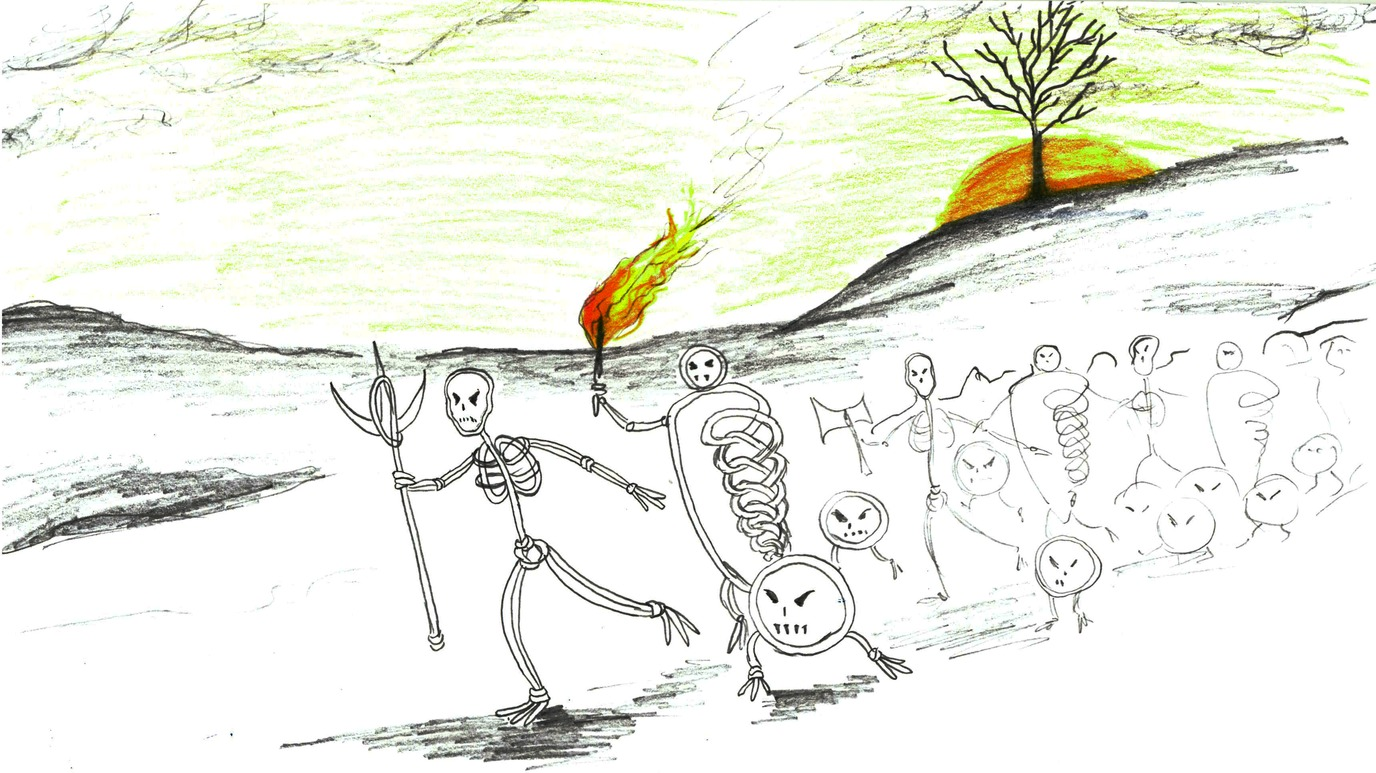
\includegraphics{knotenarmee}
\end{center}

\end{document}
